\documentclass[11pt, a4paper]{article} % use larger type; default would be 10pt

\usepackage{fontspec} % Font selection for XeLaTeX; see fontspec.pdf for documentation
\defaultfontfeatures{Mapping=tex-text} % to support TeX conventions like ``---''
\usepackage{xunicode} % Unicode support for LaTeX character names (accents, European chars, etc)
\usepackage{xltxtra} % Extra customizations for XeLaTeX
\usepackage{tikz}
\usetikzlibrary{arrows,calc,patterns}


% other LaTeX packages.....
\usepackage{fullpage}
\usepackage[top=2cm, bottom=4.5cm, left=2.5cm, right=2.5cm]{geometry}
\usepackage{amsmath,amsthm,amsfonts,amssymb,amscd,systeme}
\usepackage{unicode-math}
\usepackage{cancel}
\geometry{a4paper} 
\usepackage[parfill]{parskip} % Activate to begin paragraphs with an empty line rather than an indent
\usepackage{fancyhdr}
\usepackage{listings}
\usepackage{graphicx}
\usepackage{hyperref}
\usepackage{multicol}

% FONTS
% \setmainfont[Ligatures=TeX]{Cambria Math} % set the main body font (\textrm), assumes Charis SIL is installed
%\setsansfont{Deja Vu Sans}
% \setmonofont[Ligatures=TeX]{Fira Code}
\setmathfont[Ligatures=TeX]{NewCMMath-Regular}

\setmainfont{Cambria}
\setmonofont[Ligatures=TeX]{Roboto Mono}

\renewcommand\lstlistingname{Algorithm}
\renewcommand\lstlistlistingname{Algorithms}
\def\lstlistingautorefname{Alg.}
\lstdefinestyle{mystyle}{
    % backgroundcolor=\color{backcolour},   
    % commentstyle=\color{codegreen},
    % keywordstyle=\color{magenta},
    % numberstyle=\tiny\color{codegray},
    % stringstyle=\color{codepurple},
    basicstyle=\ttfamily\footnotesize,
    breakatwhitespace=false,         
    breaklines=true,                 
    captionpos=b,                    
    keepspaces=true,                 
    numbers=left,                    
    numbersep=5pt,                  
    showspaces=false,                
    showstringspaces=false,
    showtabs=false,                  
    tabsize=2
}
\lstset{style=mystyle}

\hypersetup{
  colorlinks   = true, %Colours links instead of ugly boxes
  urlcolor     = blue, %Colour for external hyperlinks
  linkcolor    = blue, %Colour of internal links
  citecolor   = red %Colour of citations
}


\newcommand\course{MS1 - Algebra}
\newcommand\hwnumber{Контрольна Робота 2}                   % <-- homework number
\newcommand\idgroup{111-2023}                
\newcommand\idname{Михайло Корешков}  

\usepackage[framemethod=TikZ]{mdframed}
\mdfsetup{%
	backgroundcolor = black!5,
    skipabove = 4pt,
}
\mdfdefinestyle{ans}{%
    backgroundcolor = green!5,
    linecolor = green!50,
    linewidth = 1pt,
}

\pagestyle{fancyplain}
\headheight 35pt
\lhead{\idgroup \\ \idname}
\chead{\textbf{\Large \hwnumber}}
\rhead{\course \\ \today}
\lfoot{}
\cfoot{}
\rfoot{\small\thepage}
\headsep 1.5em

\linespread{1.1}

\newcommand{\R}{\mathbb{R}}
\newcommand{\N}{\mathbb{N}}
\newcommand{\Z}{\mathbb{Z}}
\newcommand{\F}{\mathbb{F}}
\newcommand{\Q}{\mathbb{Q}}
\DeclareMathOperator{\lcm}{lcm}
\DeclareMathOperator{\cd}{CD}
\DeclareMathOperator{\ch}{char}
\DeclareMathOperator{\ob}{Ob}
\DeclareMathOperator{\mor}{Mor}
\DeclareMathOperator{\catring}{Ring}
\DeclareMathOperator{\coker}{coker}
\DeclareMathOperator{\im}{im}

\newtheorem*{proposition}{Твердження}
\newtheorem*{definition}{Визначення}

\begin{document}

\begin{mdframed}[backgroundcolor=pink!30]
    Варіант 3\\
    Завдання 2, 3, 6, 8, 9, 11, 14, 15
\end{mdframed}

% HW Ex 7.6
\section*{Ex 2}
\begin{mdframed}
    $R$ - комутативне кільце. $I$ - ідеал в $R$, $a\in R$.\\
    Нехай $J = (a) + I$. Довести, що $J/I = (a+I) \subset R/I$
\end{mdframed}
Спершу
\[J = (a) + I = \{v+y : v \in (a), y \in I\} = \{ax+y : a \in R, y \in I\}\]
Відомо, що $J$ - це ідеал, при чому найменший ідеал, що містить $(a)$ та $I$.

\[(a+I) = \{(x+I)\cdot (a+I) : x+I \in R/I\} = \{(ax)+I : x \in R\} = \{v+I : v \in (a)\}\]
\[J/I = \{u + I : u \in J\} = \{u + I : u = v+y, v \in (a), y \in I\} \]

Візьмемо вираз в фігурних дужках та зафіксуємо $y=0$. 
Матимемо $u = v \in (a)$ та 
\[(a+I) = \{v + I | v \in (a)\} \subset J/I\]

З іншого боку знаємо що $u\in I \implies (x+u) + I = x + I$.
Нехай $u+I \in J/I$.
Тоді $u \in J$. Тобто $\exists v \in (a), y \in I: u=v+y$. 
А тоді $u+I = (v + y) + I = v + I \in (a+I)$

Отже, $(a+I) \subset J/I \subset (a+I)$, з чого $(a+I) = J/I$.

А якщо коротко, то 
\[u\in I \implies (x+u) + I = x + I\]
\[(a+I) = \{v+I : v \in (a)\} = \{u+I : u = v + y, v \in (a), y \in I\} = J/I \subset R/I\]


\newpage
\section*{Ex 3}
\begin{mdframed}
    нехай $R$ - область головних ідеалів.
    Нехай $a,b\in R, \; a,b\ne 0$ не мають спільних незвідних дільників.
    
    Довести, що $(a)+(b)=(1)$
\end{mdframed}

\begin{mdframed}[backgroundcolor=purple!20]
    $R$ - область головних ідеалів.
    Тобто 

    $\forall I$ - ідеал в $R$: $\exists a\in R: I =(a)$.
    
    Також відомо, що область головних ідеалів є факторіальним кільцем, та областю цілісності.
\end{mdframed}

\begin{proof}
    
    Якщо $a$ оборотний, то $aa^{-1}=1 \in (a)$ та $(a)=(1)$, з чого одразу $(a)+(b)=(1)$.
    Надалі вважаємо, що ні $a$ ні $b$ не є оборотними.
    
    Оскільки $R$ - факторіальне кільце, то 
    \begin{align*}
        a &= p_1 \cdots p_n\\
        b &= q_1 \cdots p_m
    \end{align*}
    Де $p_i,q_i$ - різні незвідні елементи $R$.
    
    Оскільки $R$ - область головних ідеалів, нехай
    \[(a) + (b) = (s), \quad s \ne 0\]
    
    Припустимо, що $s$ - необоротний.
    $s = s_1\cdots s_t$, $s_i$ - незвідні (і тим більше необоротні).
    
    Але тоді $\exists x,y\in R:$\\
    $a+0 \in (a) + (b) = (s)$, звідки $p_1\cdots p_n = x \cdot s_1\cdots s_t$\\
    $0+b \in (a) + (b) = (s)$, звідки $q_1\cdots q_m = y \cdot s_1\cdots s_t$\\
    
    Тобто, $a,b$ мають спільні множники, що суперечить умові.
    А тоді припущення, що $s$ необоротний неправдиве, отже $s$ - оборотне, з чого
    \[(a) + (b) = (1)\]
\end{proof}

\newpage
\section*{Ex 6}
\begin{mdframed}
    Довести що $f(x) = 7x^3 + 6x^2 + 4x + 6$ є незвідним в $\Q[x]$ трьома способами
\end{mdframed}

$\Q$ - поле.
$\Q[x]$ - евклідове кільце (область головних ідеалів, факторіальне кільце).

Контент $\operatorname{cont} f(x) = K = \gcd(7,6,4,6) = 1$, бо 7 - просте. 
Тобто поліном $f(x)$ - примітивний.   

З наслідку 9.28 випливає, що $f(x)$ незвідний в $\Q[x]$ тоді і лише тоді коли він незвідний в $\Z[x]$.

\subsection*{1 спосіб}
$\deg f = 3$. Перевірка на раціональні корені.

Нехай $f(\frac{p}{q}) = 0$.
Тоді $p\mid 7, q \mid 6$.

\[c \in \{ \pm 1, \pm 1/2, \pm 1/3, \pm 1/6, \pm 7, \pm 7/2, \pm 7/3, \pm 7/6\}\]
\begin{figure}[h]
    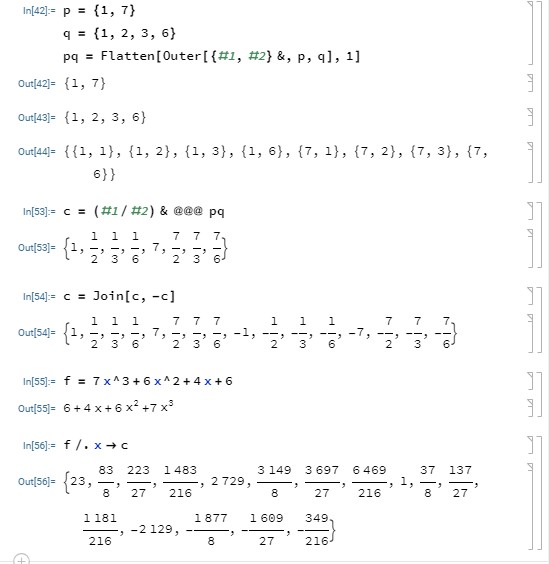
\includegraphics[width=0.6\textwidth]{6.1.png}
    \centering
\end{figure}

Бачимо, що жоден можливий корінь не підходить. 
Разом з $\deg f \le 3$ та Зауваження 9.31 випливає, що $f$ - незвідний в $\Z$.

\newpage
\subsection*{2 спосіб}
\begin{itemize}
    \item $2\nmid 7$. $\underline{f(x)}_2 = 1x^3+0x^2+0x+0 = x^3 \in (\Z/2\Z)[x]$. Цей поліном не є незвідним.
    \item $2\nmid 7$. $\underline{f(x)}_2 = 1x^3+0x^2+0x+0 = x^3 \in (\Z/2\Z)[x]$. Цей поліном не є незвідним.
    \item $5\nmid 7$. $\underline{f(x)}_5 = 2x^3+1x^2-1x+1 \in (\Z/5\Z)[x]$.\\
    $\underline{f(0)}_5 = 1, \underline{f(1)}_5 = 3, \underline{f(2)}_5 = 4, \underline{f(3)}_5 = 1, \underline{f(4)}_5 = 1$\\
\end{itemize}
З того, що $(\Z/5\Z)$ - це поле, $\deg \underline{f(x)}_5=3$, відсутності коренів, та Твердження 9.18 маємо, 
що $\underline{f(x)}_5$ - незвідний.
А з Твердження 9.33 маємо, що $f(x)$ - незвідний в $\Z[x]$.

\subsection*{3 спосіб}
$f(x) = 7x^3 + 6x^2 + 4x + 6$. $\deg f(x) \ge 1$.
\begin{enumerate}
    \item $2 \nmid 7$
    \item $2 \mid 6,4,6$
    \item $2^2=4 \nmid 6$
\end{enumerate}

Застосовний критерій Ейзенштейна (Теорема 9.35), внаслідок якого $f(x)$ незвідний в $\Q[x]$.

\newpage
\section*{Ex 8}
\begin{mdframed}
    $R$ - кільце. $M,N$ - прості $R$-модулі ($S$-підмодуль $M \implies S=\{0\} \vee S=M$).\\
    Нехай $f : M \to N$ - гомоморфізм.

    Довести, що $f = 0$ або $f$ - ізоморфізм.
\end{mdframed}
\begin{proof}
    \[f(a+b) = f(a)+f(b), \quad f(ra)=rf(a)\]

    $f(\{0\})$ буде підмодулем $N$.
    Значить $f(0_M)=0_N$.

    $f(M)$ буде підмодулем $N$.
    Значить $f(M) = \{0\}$ або $f(M) = N$.

    Далі вважаємо, що $f \ne 0$.
    
    Повний прообраз $f^{-1}(0)$ має бути підмодулем $M$. 
    Оскільки $f\ne 0$, то $f^{-1}(0)=\{0\}$.

    $f(M)=N$ також означає, що $f$ - сюр'єктивне.
    Припустимо, що $f(x)=f(y)=a$.
    Тоді $f(x)-f(y) = f(x-y) = 0$.
    $f^{-1}(0) = \{0\}$, значить $x=y$. Таким чином довели ін'єктивність.

    Отже, $f$ - нульове або бієктивний гомоморфізм, тобто ізоморфізм.
\end{proof}

\section*{Ex 9}
\begin{mdframed}
    Підрахувати коядро гомоморфізма $f:\Z^{\oplus 3}\to\Z^{\oplus 3}$, що визначається матрицею
    \[A = \begin{pmatrix}
        0 & -2 & 0 \\
        6 & 4 & -2 \\
        2 & 4 & 2
    \end{pmatrix}\]
\end{mdframed}

$\coker f := N / \im f$

Приведемо матрицю $A$ до більш простого вигляду за допомогою елементарних операцій.
\begin{align*}
    A &= \begin{pmatrix}
        0 & -2 & 0 \\
        6 & 4 & -2 \\
        2 & 4 & 2
    \end{pmatrix} \sim
    \begin{pmatrix}
        0 & -2 & 0 \\
        6 & 0 & -2 \\
        2 & 0 & 2
    \end{pmatrix} \sim
    \begin{pmatrix}
        0 & -2 & 0 \\
        4 & 0 & -2 \\
        0 & 0 & 2
    \end{pmatrix} \sim
    \begin{pmatrix}
        0 & -2 & 0 \\
        4 & 0 & 0 \\
        0 & 0 & 2
    \end{pmatrix} \sim \\
    &\sim \begin{pmatrix}
        4 & 0 & 0 \\
        0 & -2 & 0 \\
        0 & 0 & 2
    \end{pmatrix} = A'
\end{align*}

Матриця $A'$ визначає гомоморфізм $f' : \Z^{\oplus 3}\to\Z^{\oplus 3}$.
\[f'(x,y,z) = (4x,-2y,2z)\]
\[\im f' = <4> \oplus <-2> \oplus <2> = 4\Z \oplus 2\Z \oplus 2\Z \]
\[\coker f' = (\Z\oplus\Z\oplus\Z)/(4\Z \oplus 2\Z \oplus 2\Z) \cong \Z_4\oplus\Z_2\oplus\Z_2\]

Отже, $\coker f \cong \Z_4\oplus\Z_2\oplus\Z_2$

\section*{Ex 11}
\begin{mdframed}
    Нехай $R$ - кільце Нетер. Нехай $M$ - скінченно породжений $R$-модуль.

    Довести, що кожен підмодуль $M$ є скінченно породженим.
\end{mdframed}
\begin{proof}
    Нехай $M$ - скінченно породжений $R$-модуль. З Теореми 11.31, він також скінченно представлений.
    Тобто існує вільні модулі скінченного рангу $R^{\oplus m}, R^{\oplus n}$ 
    такі що справедлива точна послідовність 
    \[R^{\oplus m} \overset{g}{\longrightarrow} R^{\oplus n} \overset{f}{\longrightarrow} M \longrightarrow 0\].

    Нехай $S$ - підмодуль $M$.
    Відомо, що $T = f^{-1}(S)$ буде підмодулем $R^{\oplus n}$. 
    З Леми 11.34, він буде скінченно породженим.
    Тобто справедлива точна послідовність
    \[R^{\oplus m_1} \overset{g}{\longrightarrow} T \longrightarrow 0\]
    Тобто $\im g = T$.

    А тоді справедлива точна послідовність
    \[R^{\oplus m_1} \overset{f\circ g}{\longrightarrow} S \longrightarrow 0\].

    Перевірю:\\
    $\im f\circ g = f(\im g) = f(T) = S$

    Отже, $S$ - скінченно породжений.
\end{proof}


\section*{Ex 14}
\begin{mdframed}
    Виписати всі елементи групи $S_4$ у вигляді добутків незалежних циклів.

    Які з них належать до знакозмінної підгрупи $A_4$?
\end{mdframed}

\[S_4 \cong Aut_{Set}(\{1,2,3,4\})\]
\[|S_4| = 4! = 24\]

Знайдемо всі представлення 24 через інваріантні множники:\\
\begin{align*}
    24 &=  2^3\cdot 3 \\
    &= 2 \cdot 12 
\end{align*}
Інших представлень немає.
Значить єдині два представлення $S_4$ через циклічні групи це 
\[S_4 \cong C_{24} \cong C_{2} \oplus C_{12}\] 

\begin{enumerate}
    \item $\begin{pmatrix}
        1 &2 &3 &4\\
        1 &2 &3 &4
    \end{pmatrix} = (1)(2)(3)(4)$. $\sigma = 1\cdot 1 \cdot 1 \cdot 1 = 1$. $\in A_4$.
    \item $\begin{pmatrix}
        1 &2 &3 &4\\
        1 &2 &4 &3
    \end{pmatrix} = (1)(2)\begin{pmatrix}3 & 4\end{pmatrix}$.
    $\sigma = 1\cdot 1 \cdot (-1) = -1$

    \item $\begin{pmatrix}
        1 &2 &3 &4\\
        1 &3 &2 &4
    \end{pmatrix} = (1)\begin{pmatrix}2 &3\end{pmatrix}(4)$.
    $\sigma = 1\cdot (-1) \cdot 1 = -1$

    \item $\begin{pmatrix}
        1 &2 &3 &4\\
        1 &3 &4 &2
    \end{pmatrix} = (1)\begin{pmatrix}2 &3 &4\end{pmatrix}$.
    $\sigma = 1\cdot 1 = 1$. $\in A_4$

    \item $\begin{pmatrix}
        1 &2 &3 &4\\
        1 &4 &2 &3
    \end{pmatrix} = (1)\begin{pmatrix}2 &4 &3\end{pmatrix}$.
    $\sigma = 1\cdot 1 = 1$. $\in A_4$

    \item $\begin{pmatrix}
        1 &2 &3 &4\\
        1 &4 &3 &2
    \end{pmatrix} = (1)\begin{pmatrix}2 &4\end{pmatrix}(3)$.
    $\sigma = 1 \cdot (-1) \cdot 1 = -1$

    \item $\begin{pmatrix}
        1 &2 &3 &4\\
        2 &1 &3 &4
    \end{pmatrix} = \begin{pmatrix}1 &2\end{pmatrix}(3)(4)$.
    $\sigma = (-1) \cdot 1 \cdot 1 = -1$

    \item $\begin{pmatrix}
        1 &2 &3 &4\\
        2 &1 &4 &3
    \end{pmatrix} = \begin{pmatrix}1 &2\end{pmatrix}\begin{pmatrix}3 &4\end{pmatrix}$.
    $\sigma = (-1) \cdot (-1) = 1$. $\in A_4$

    \item $\begin{pmatrix}
        1 &2 &3 &4\\
        2 &3 &1 &4
    \end{pmatrix} = \begin{pmatrix}1 &2 &3\end{pmatrix}(4)$.
    $\sigma = 1 \cdot 1 = 1$. $\in A_4$

    \item $\begin{pmatrix}
        1 &2 &3 &4\\
        2 &3 &4 &1
    \end{pmatrix} = \begin{pmatrix}1 &2 &3 &4\end{pmatrix}$.
    $\sigma = -1$

    \item $\begin{pmatrix}
        1 &2 &3 &4\\
        2 &4 &1 &3
    \end{pmatrix} = \begin{pmatrix}1 &2 &4 &3\end{pmatrix}$.
    $\sigma = -1$

    \item $\begin{pmatrix}
        1 &2 &3 &4\\
        2 &4 &3 &1
    \end{pmatrix} = \begin{pmatrix}1 &2 &4\end{pmatrix}(3)$.
    $\sigma = 1 \cdot 1 = 1$. $\in A_4$

    \item $\begin{pmatrix}
        1 &2 &3 &4\\
        3 &1 &2 &4
    \end{pmatrix} = \begin{pmatrix}1 &3 &2\end{pmatrix}(4)$.
    $\sigma = 1 \cdot 1 = 1$. $\in A_4$

    \item $\begin{pmatrix}
        1 &2 &3 &4\\
        3 &1 &4 &2
    \end{pmatrix} = \begin{pmatrix}1 &3 &4 &2\end{pmatrix}$.
    $\sigma = -1$

    \item $\begin{pmatrix}
        1 &2 &3 &4\\
        3 &2 &1 &4
    \end{pmatrix} = \begin{pmatrix}1 &3\end{pmatrix}(2)(4)$.
    $\sigma = (-1) \cdot 1 \cdot 1 = -1$

    \item $\begin{pmatrix}
        1 &2 &3 &4\\
        3 &2 &4 &1
    \end{pmatrix} = \begin{pmatrix}1 &3 &4\end{pmatrix}(2)$.
    $\sigma = 1 \cdot 1 = 1$. $\in A_4$

    \item $\begin{pmatrix}
        1 &2 &3 &4\\
        3 &4 &1 &2
    \end{pmatrix} = \begin{pmatrix}1 &3\end{pmatrix}\begin{pmatrix}2 &4\end{pmatrix}$.
    $\sigma = (-1) \cdot (-1) = 1$. $\in A_4$

    \item $\begin{pmatrix}
        1 &2 &3 &4\\
        3 &4 &2 &1
    \end{pmatrix} = \begin{pmatrix}1 &3 &2 &4\end{pmatrix}$.
    $\sigma = -1$

    \item $\begin{pmatrix}
        1 &2 &3 &4\\
        4 &1 &2 &3
    \end{pmatrix} = \begin{pmatrix}1 &4 &3 &2\end{pmatrix}$.
    $\sigma = -1$

    \item $\begin{pmatrix}
        1 &2 &3 &4\\
        4 &1 &3 &2
    \end{pmatrix} = \begin{pmatrix}1 &4 &2\end{pmatrix}(3)$.
    $\sigma = 1 \cdot 1 = 1$. $\in A_4$

    \item $\begin{pmatrix}
        1 &2 &3 &4\\
        4 &2 &1 &3
    \end{pmatrix} = \begin{pmatrix}1 &4 &3\end{pmatrix}(2)$.
    $\sigma = 1 \cdot 1 = 1$. $\in A_4$

    \item $\begin{pmatrix}
        1 &2 &3 &4\\
        4 &2 &3 &1
    \end{pmatrix} = \begin{pmatrix}1 &4\end{pmatrix}(2)(3)$.
    $\sigma = (-1) \cdot 1 \cdot 1 = -1$

    \item $\begin{pmatrix}
        1 &2 &3 &4\\
        4 &3 &1 &2
    \end{pmatrix} = \begin{pmatrix}1 &4 &2 &3\end{pmatrix}$.
    $\sigma = -1$

    \item $\begin{pmatrix}
        1 &2 &3 &4\\
        4 &3 &2 &1
    \end{pmatrix} = \begin{pmatrix}1 &4\end{pmatrix}\begin{pmatrix}2 &3\end{pmatrix}$.
    $\sigma = (-1) \cdot (-1) = 1$. $\in A_4$
\end{enumerate}

В сумі $|A_4|=12 \mid 24$, як і має бути. 


\newpage
\section*{Ex 15}
\begin{mdframed}
    Нехай $G$ - скінченна група, $H,K$ - її підгрупи.
    Нехай $H\cap K = \{e\}$.
    
    Довести, що $|HK|=|H|\cdot |K|$, де $HK = \{hk : h\in H, k \in K\}$.
\end{mdframed}
\begin{proof}
    Нехай $A = H \times K$ - прямий добуток підгруп з операцією $(a,b)\cdot (x,y) = (ax,by)$.

    Нехай $f : A \to G$, $f(h,k) = hk$, $f$ - \textbf{не} гомоморфізм.
    Зверну увагу що $f(A) = HK$, тобто це сюр'єкція.

    Оберемо довільний $a \in HK$, $a = hk, h \in H, k \in K$.\\
    Тоді $\forall x \in H \times K: \exists u\in H, v \in K: x = (hu,vk)$.
    Звідси $f(x) = f(hu,vk) = huvk$.

    Нехай $f(x) = a$. Тоді $huvk = a = hk$. Це можливо лише якщо $uv=1$, тобто $v=u^{-1}$ та $u\in H\cap K$.\\
    Але $H\cap K = \{e\}$, отже $(f(x) = a) \implies x = (h,k)$.
    
    Оскільки ми брали довільний $a \in HK$, можна зробити висновок, що $f$ - ін'єктивне відображення.
    Отже, маємо бієкцію $f$ між скінченними множинами.
    З цього, 
    \[|HK| = |H\times K| = |H|\cdot |K|\]
\end{proof}





\end{document}

